\documentclass[14pt]{extarticle}
\usepackage{graphicx}
\usepackage{amsmath}
\usepackage{xcolor}





\begin{document}

\title{Organizzazione e Gestione per lo startup Aziendale}
\author{Alessandro Savioli}
\date{Febbraio 2025}

\maketitle

\tableofcontents

\newpage

\section{Lezione 1}

\section{Lezione 2}

\section{Lezione 3}
\subsection{La Struttura Organizzativa}

\textbf{Organizzare} significa ordinare un sistema di parti dipendenti tra loro,
definendo per ognuna uno specifico ruolo all'interno del sistema stesso.

Per fare ciò, serve trovare una \textcolor{red}{Struttura Organizzativa}, in cui
possiamo trovare:
\begin{enumerate}
    \item Un insieme di relazioni tra le persone interne all'azienda;
    \item Una distribuzione delle Autorità e delle Responsabilità;
    \item Un insieme di processi con i quali l'azienda si costituisce.
\end{enumerate}
Questa struttura non può essere formulata partendo da un modello ideale ed
astratto, bensì deve essere \textbf{adattata} alla realtà nella quale l'azienda
opera.

Una struttura organizzativa è composta da elementi:
\begin{itemize}
    \item \textbf{Hardware (o di struttura)} meccanismo attraverso il quale
    vengono affidate delle funzioni a tutte le parti del sistema;
    \item \textbf{Software (o decisionali)} che stabilisce scopo, finalità e \\
    obiettivi dell'organizzazione e ne elabora le norme e le relazioni delle
    parti.  
\end{itemize}
Inoltre, una struttura organizzativa può essere di tipo:

\begin{itemize}
    \item \textbf{Formale}, dove la divisione in mansioni e la loro integrazione
    è esplicitamente riconosciuta e può essere rappresentata tramite gli
    \textbf{organigrammi};
    \item \textbf{Informale}, che fa riferimento a rapporti spontanei e a
    fattori di influenza e potere. 
\end{itemize}

\subsection{Gli Organigrammi}

Gli organigrammi sono delle rappresentazioni grafiche globali, di facile
comprensione, della struttura organizzativa formale dell'impresa.

Il loro scopo è quello di evidenziare gli aspetti fondamentali del funzionamento
dell'organizzazione, le posizioni strutturali ed i collegamenti tra le diverse
funzioni aziendali.
\begin{center}
    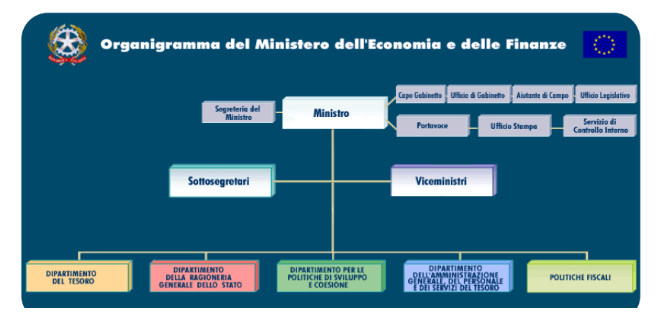
\includegraphics[scale = 0.80]{images/Esempio_Organigramma}
    Esempio di un organigramma 
\end{center}
Questo tipo di rappresentazione grafica ha però dei difetti, in quanto si fa
difficoltà a capire l'importanza delle posizioni rappresentate, non si hanno
informazioni sui rapporti non gerarchici e non si capisce in che ambiente opera
l'azienda.

\subsection{I vari Tipi di Struttura Organizzativa}
\subsubsection{Il modello Gerarchico (Struttura Monofunzionale)}

\begin{center}
    \textcolor{red!50}{CARATTERISTICHE}
\end{center}


\begin{itemize}
    \item \textbf{Principio di gerarchia}, secondo il quale \\ autorità,
    responsabilità e le competenze sono massime al vertice dell'organizzazione;
    \item \textbf{Principio di delega}, secondo il quale le funzioni vengono
    delegate verso il basso;
    \item \textbf{Principio di eccezione}, secondo il quale, in caso di
    difficoltà impreviste il problema deve tornare al vertice per essere
    risolto;
    \item \textbf{Principio dell'unità di direzione}, secondo il quale ciascuno
    deve aver ben chiaro da chi prendere ordini e a chi rivolgersi quando non
    sia in grado di decidere da solo.  
\end{itemize}

\begin{center}
    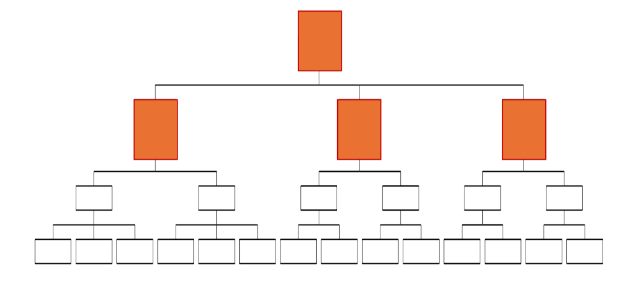
\includegraphics[scale = 0.80]{images/modello_gerarchico}
    Esempio di modello gerarchico
\end{center}

\newpage

\subsubsection{Il modello Gerarchico Funzionale (Struttura Gerarchico Funzionale)}

\begin{center}
    \textcolor{red!50}{CARATTERISTICHE}
\end{center}

Questo modello presenta attività raggruppate in base ad una funzione comune ed
esalta il \textbf{principio della specializzazione} delle singole aree.

Continua a seguire il \textbf{Principio di gerarchia} ed il \textbf{Principio di
eccezione} dal modello precedente.

\begin{center}
    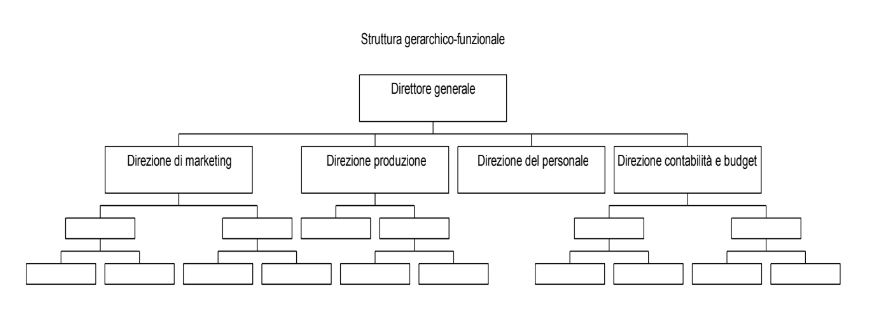
\includegraphics[scale = 0.64]{images/modello_gerarchico_funzionale}
    Esempio di modello gerarchico funzionale
\end{center}
Nella struttura gerarchico funzionale esistono tre livelli organizzativi
fondamentali:

\begin{enumerate}
    \item \textbf{Direzione generale}, a cui è affidato il compito di
    amministrare l'azienda tramite una visione d'insieme che permetta di
    definire gli obiettivi primari e coordinare le diverse aree funzionali;
    \item \textbf{Direzioni dei dipartimenti funzionali}, che sono specializzate
    nelle varie funzioni, quindi non in grado di occuparsi di problemi generali,
    ma solo di problemi settoriali;
    \item \textbf{Unità operative}, ovvero organi che fanno capo ai dipartimenti
    funzionali, per realizzare piani predisposti da quest'ultimi, hanno compiti
    prevalentemente esecutivi. 
\end{enumerate}

Le principali direzioni funzionali sono:

\begin{itemize}
    \item \textbf{Direzione Marketing};
    \item \textbf{Direzione della Produzione};
    \item \textbf{Direzione del Personale};
    \item \textbf{Direzione Amministrativa};
    \item \textbf{Direzione Finanza};
    \item \textbf{Direzione Ricerca e Sviluppo};
\end{itemize}

un esempio di modello gerarchico funzionale può essere identificato nel modello
strutturale utilizzato da Apple.

\subsubsection{Il modello Divisionale}

In questo modello vengono organizzate divisioni separate, ciascuna è
responsabile di un singolo prodotto, servizio o programma principale. Questa
struttura è anche denominata \textbf{struttura per prodotto}.

\begin{center}
    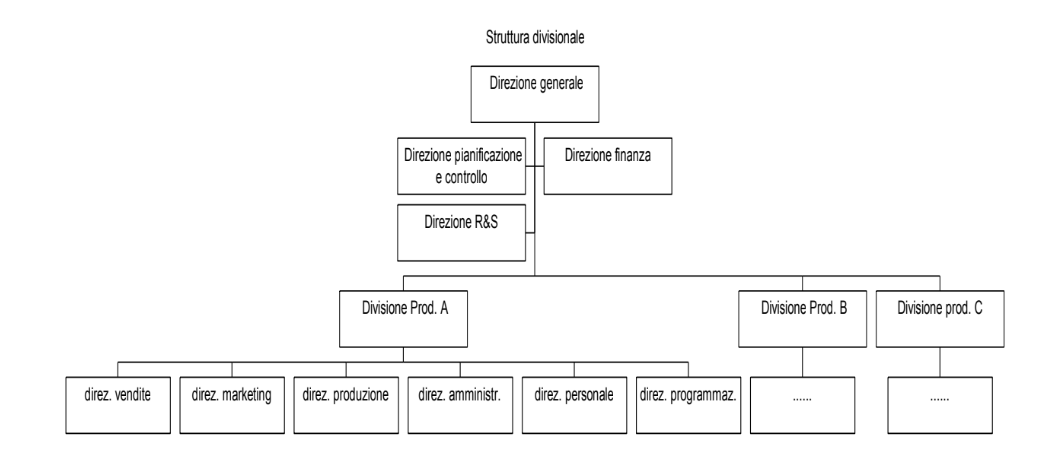
\includegraphics[scale = 0.50]{images/modello_divisionale.png}
    Esempio di modello divisionale
\end{center}

Un'azienda che adopera il modello divisionale è \textbf{Alphabet}, proprietaria
di Google.

\subsubsection{Il modello per Area Geografica}

Questo modello risulta simile al modello divisionale, con l'unica differenza che
le divisioni sono organizzate per area geografica. Questo tipo di struttura
aiuta l'azienda ad espandersi in nuovi mercati e a fare un uso più efficiente
delle risorse.

\begin{center}
    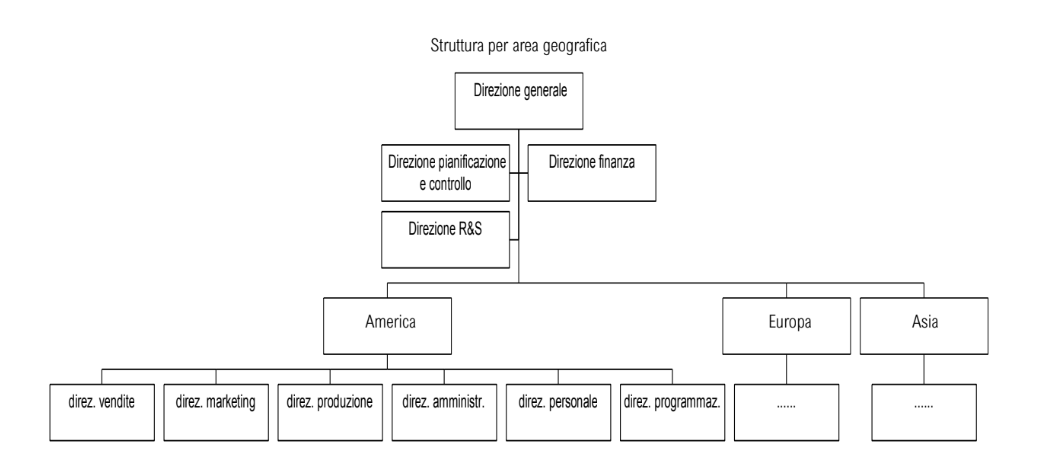
\includegraphics[scale=0.50]{images/modello_geografico.png}
    Esempio di modello per area geografica
\end{center}

\subsubsection{Il modello a Matrice}

Questo modello cerca di combinare al meglio i vantaggi dell' \\ 
organizzazione per funzioni con quelli dell'organizzazione per prodotti o
progetti.

\begin{center}
    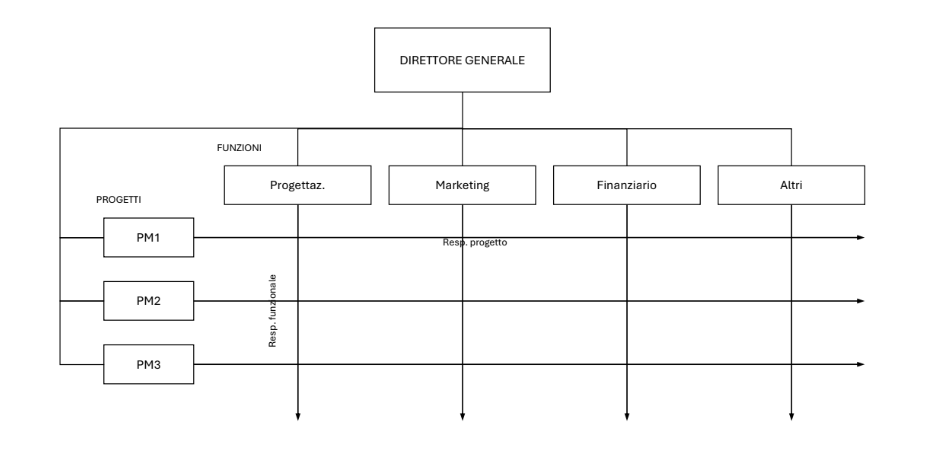
\includegraphics[scale=0.60]{images/modello_matrice.png}
    Esempio di modello a matrice
\end{center}
Molte aziende adoperano questo tipo di struttura, tra le più celebri troviamo
Intel, Spotify, Microsoft, IBM, Philips.

\subsubsection{Il modello a Rete}

Questo modello affida varie parti dell'organizzazione a partner esterni. In
questo caso si parla di \textbf{Outsourcing}, ovvero quando l'azienda ricorre a
fornitori esterni per determinati compiti o funzioni, quali la produzione, le
risorse umane o la gestione dei crediti.

\begin{center}
    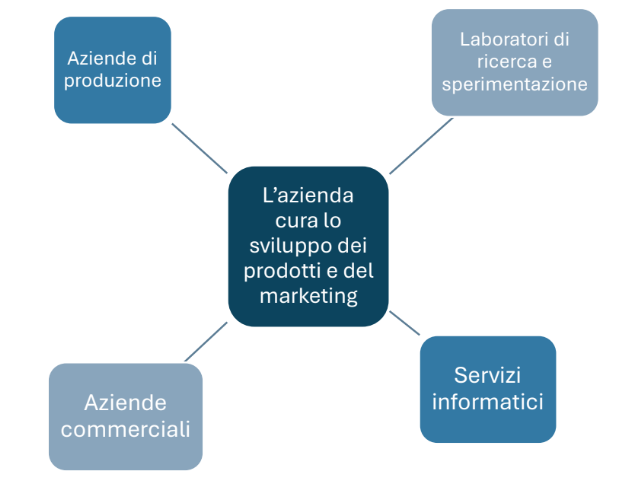
\includegraphics[scale=0.80]{images/modello_rete.png}
\end{center}
Un grande esempio di azienda che adopera questa struttura è Nike, che affida la
produzione e la distribuzione dei propri prodotti ad aziende esterne.

\section{Lezione 4}

\subsection{Stadi dello Sviluppo di un'azienda}

In questo capitolo andremo ad osservare i vari stadi dello sviluppo di
un'azienda, le varie crisi e le soluzioni che vengono adottate per poter
progredire.

\subsubsection{Stadio imprenditoriale}

Quando un'impresa è ancora allo stato embrionale, l'enfasi è posta sulla
\textbf{creazione} di un prodotto o un servizio e sulla \textbf{sopravvivenza}
nel mercato. L'organizzazione in questo momento risulta informale e non
burocratica, vi è un controllo diretto da parte del proprietario.

\begin{center}
    \textcolor{red!50}{Crisi: Bisogno di leadership}

    man mano che l'organizzazione cresce con l'aumento del numero dei dipendenti
    vengono a crearsi problemi relativi alla gestione, gli imprenditori si
    trovano costretti ad adattare una struttura organizzativa per assecondare un
    processo continuo di crescita.
\end{center}

\subsubsection{Stadio della collettività}

Se la crisi di leadership viene superata, si ottiene una direzione forte e
inizia lo sviluppo di obiettivi e di una direzione chiara dell'azienda. Vengono
strutturate le unità organizzative insieme ad una gerarchia di autorità, vengono
definiti i compiti e una prima divisione del lavoro. In questo stadio i
dipendenti cominciano ad \textbf{identificarsi} nella missione
dell'organizzazione ed idealmente dedicano molto tempo a contribuire al successo
organizzativo. La comunicazione e il controllo continuano ad essere
prevalentemente informali, comincia a nascere qualche sistema formale

\begin{center}
    \textcolor{red!50}{Crisi: Bisogno di delega}

    se il management ha operato con successo, i dipendenti a livelli inferiori
    si trovano limitati dalla forte leadership esercitata dall'alto, d'altra
    parte i manager di livello inferiore cominciano a chiedere una maggiore
    fiducia, l'organizzazione si trova dunque a dover escogitare un meccanismo
    per coordinare le diverse unità senza la supervisione del vertice.
\end{center}

\subsubsection{Stadio della formalizzazione}

Vengono introdotte nuove regole, procedure e sistemi di controllo. La
comunicazione diviene formale e segue la linea gerarchica. La direzione comincia
ad interessarsi maggiormente a strategia e pianificazione lasciando gli aspetti
produttivi ad un livello più basso di management.

\begin{center}
    \textcolor{red!50}{Crisi: Eccesso di burocrazia}

    Lo sviluppo dell'organizzazione porta ad una proliferazione di sistemi e
    procedure che possono cominciare a soffocare i manager dei livelli
    intermedi. L'organizzazione risulta troppo grande e complessa per essere
    gestita da programmi formali.
\end{center}

\subsubsection{Stadio di elaborazione}

La soluzione all'ultima crisi consiste nel far raggiungere alla burocrazia il
suo limite superiore (oltre il quale avremmo un eccesso), i manager imparano a
lavorare all'interno della burocrazia senza doverla accrescere. In questi casi
l'azienda può anche essere scomposta in divisioni per mantenere la filosofia da
piccola azienda.

\begin{center}
    \textcolor{red!50}{Crisi: Bisogno di rivitalizzazione}

    Dopo che l'azienda ha raggiunto la maturità è possibile che si cominci a
    manifestare un bisogno di rinnovamento, che può essere sentito con cadenze
    che vanno dai 10 ai 20 anni. L'azienda si disallinea rispetto all'ambiente
    in cui opera o diventa lenta e troppo burocratica, deve passare attraverso
    uno stadio di snellimento e innovazione.
\end{center}

\begin{center}
    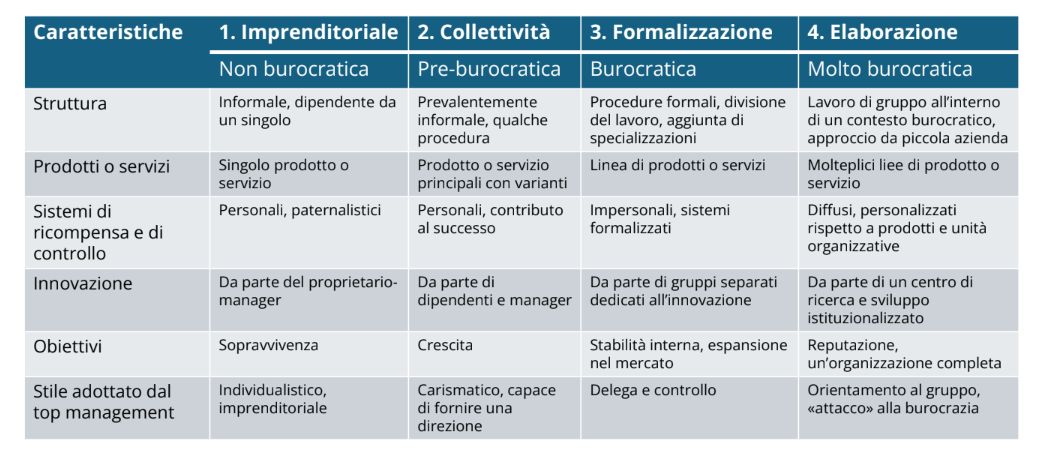
\includegraphics[scale=0.50]{images/stati_sviluppo.png}
    Mappa degli stadi di sviluppo
\end{center}

\subsection{Stadi del Declino di un'azienda}

Sulla base di un ampio studio sul declino organizzativo è stato \\
proposto un modello che attraversa 5 stadi fino alla \textbf{dissoluzione}
dell'organizzazione.

\subsubsection{Stadio della cecità}

Essendo il primo stadio, risulta complesso per il management avvertire i segnali
di declino, che possono presentarsi sotto forma di:

\begin{enumerate}
    \item Personale in eccesso;
    \item Procedure troppo complesse;
    \item Mancanza di allineamento con il proprio target;
    \item Ecc. 
\end{enumerate}
La soluzione per prevenire questo stato di \textbf{cecità} è mettere \\ in campo
sistemi di monitoraggio e di controllo che indichino prontamente quando qualcosa
non funziona, infatti potendo contare su informazioni tempestive il management
può riportare l'organizzazione alle prestazioni ottimali.

\subsubsection{Stadio dell'inattività}

Questo stadio deriva da una mancata attenzione alle condizioni correnti di
declino malgrado eventuali segni di calo delle prestazioni. La soluzione per
prevenire l'\textbf{inattività} è riconoscere l'eventuale declino e
intraprendere azioni rapide per riallineare l'organizzazione. Queste azioni
possono comprendere:

\begin{enumerate}
    \item Nuovi approcci alla risoluzione dei problemi;
    \item Maggiore partecipazione al processo decisionale;
    \item Incoraggiamento delle manifestazioni di insoddisfazione da parte dei
    dipendenti e dei clienti per capire cosa non funziona.   
\end{enumerate}

\subsubsection{Stadio dell'errore}

In questo stadio l'organizzazione affronta i problemi gravi e gli indicatori che
mostrano che i cattivi risultati non possono più essere ignorati. Il management
è quindi costretto a ricorrere a cambiamenti drastici.

Le possibilità per far fronte a questa situazione possono essere:

\begin{enumerate}
    \item Ridurre i costi, tagliando il personale;
    \item Ridurre l'incertezza dei dipendenti chiarendo valori e fornendo
    informazioni;  
\end{enumerate}

Un errore commesso in questo stadio può sancire il \textbf{punto di non ritorno}
per l'organizzazione.

\subsubsection{Stadio della crisi}

A questo punto non si è stati ancora in grado di gestire in modo efficace il
declino e ci si trova in una situazione di panico. L'unica soluzione è una
\textbf{radicale riorganizzazione}. Vengono intraprese soluzioni drastiche, come
la sostituzione del management, rivoluzioni a livello di struttura, strategia e
cultura. In questo caso il taglio della forza lavoro può essere molto severo.

\subsubsection{Stadio della dissoluzione}

Questo stadio risulta irreversibile. L'organizzazione subisce perdite ingenti di
quote di mercato e di reputazione, dei suoi migliori talenti e dei capitali.
L'unica azione possibile è quella di porre fine all'organizzazione in maniera
ordinata.

\begin{center}
    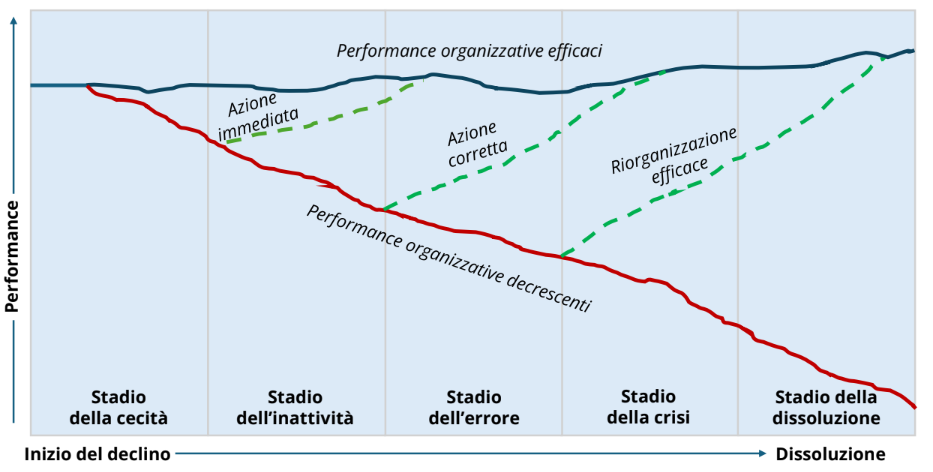
\includegraphics[scale=0.60]{images/stadi_declino.png}
    Mappa degli stadi del declino
\end{center}

\newpage
\subsection{I diversi tipi di Azienda in Italia}

Secondo l'articolo 2555 del codice civile l'azienda è \textbf{il complesso dei
beni organizzati dall'imprenditore per l'esercizio dell'impresa}. Vediamo
insieme due tipi di azienda:

\begin{itemize}
    \item \textbf{Aziende di produzione (imprese profit)}, che rendono \\
    disponibili i loro prodotti o servizi per il consumo o per altre imprese
    mediante lo scambio di mercato; 
    \item \textbf{Aziende di erogazione (corporazioni, fondazioni)}, che
    soddisfano i bisogni di determinati soggetti (associati, affiliati,
    fondatori) direttamente.
    \begin{itemize}
        \item \textbf{Corporazioni}, in cui è prevalente l'elemento personale.
        Mediante la raccolta dei contributi degli associati riescono a
        soddisfare i propri bisogni;
        \item \textbf{Fondazioni}, in cui è prevalente l'aspetto patrimoniale.
        Sorgono in virtù di lasciti o donazioni per raggiungere determinati
        scopi individuali e di utilità sociale. 
    \end{itemize} 
\end{itemize}

\subsubsection{La ditta individuale o società}

Le aziende di produzione possono essere esercitate in:

\begin{itemize}
    \item \textbf{Forma individuale}
    \item \textbf{Forma collettiva, ovvero in società} 
\end{itemize}

\newpage
Nella \textbf{Ditta individuale} il titolare risponde illimitatamente delle
obbligazioni contratte dall'azienda, indipendentemente dalla parte del suo
patrimonio investita nella ditta stessa.

\begin{center}
    \textbf{Vantaggi}:

    imposizione fiscale unica, contabilità semplice, gestione poco costosa.

    \textbf{Svantaggi}:

    Responsabilità illimitata.
\end{center}

Secondo l'articolo 2247 del codice civile:
\begin{center}
    \textbf{con il contratto di società due o più persone conferiscono beni o
servizi per l'esercizio comune di un'attività economica allo scopo di dividerne
gli utili}
\end{center}

Abbiamo due tipi di società differenti:

\begin{itemize}
    \item \textbf{Società di persone}, come s.s., s.n.c., s.a.s., che hanno una
    gestione poco onerosa ma allo stesso tempo hanno una responsabilità
    economica illimitata;
    \item \textbf{Società di capitali}, come s.p.a., s.a.p.a., s.r.l., s.r.l.s,
    che hanno una responsabilità \\
    limitata ma per questo ottengono un'imposizione fiscale doppia, con
    conseguente gestione onerosa. 
\end{itemize}

\subsection{Il bilancio di un'azienda}

Il bilancio d'esercizio è un documento informativo per un insieme eterogeneo di
soggetti, risulta utile per determinare il reddito d'esercizio e il capitale di
funzionamento, ovvero darci un'idea di come stia andando l'azienda.

TUTTE le aziende sono obbligate a redigere annualmente il bilancio ma con
modalità differenti:

\begin{itemize}
    \item \textbf{Società di capitali}: Il bilancio deve essere compilato
    seguendo uno schema a struttura obbligatoria e deve essere reso pubblico; 
    \item \textbf{Società di persone}: Il bilancio può essere presentato in
    forma libera e non è soggetto a pubblicazione. 
\end{itemize}

\subsubsection{Elementi di un bilancio d'esercizio}

Il bilancio di esercizio di una società è composto dai seguenti elementi:

\begin{enumerate}
    \item Lo \textbf{Stato patrimoniale};
    \item Il \textbf{Conto economico};
    \item La \textbf{Nota integrativa}.
\end{enumerate}

Lo \textcolor{red}{stato patrimoniale} rappresenta la situazione patrimoniale e
finanziaria della \\
società. In quest'ultimo vengono indicate le attività, passività e il patrimonio
netto della società alla data di chiusura dell'esercizio.

Il \textcolor{red}{conto economico} evidenzia il risultato economico
dell'esercizio, fornisce una rappresentazione delle operazioni di gestione,
sintetizzando componenti positivi e negativi di reddito che hanno contribuito al
risultato economico.

La \textcolor{red}{nota integrativa} costituisce parte integrante del bilancio,
fornendo informazioni aggiuntive ai dati presenti nei due punti precedenti.

\newpage
\subsection{l'Analisi di bilancio}

L'analisi di bilancio serve a monitorare lo stato di salute di un'impresa. Per
potere analizzare correttamente un bilancio, serve prima
\textbf{riclassificarlo}, per poter:

\begin{enumerate}
    \item Rendere omogenei i dati di bilancio;
    \item far emergere alcune informazioni non immediate.
\end{enumerate}

\section{Lezione 5}

\subsection{La start-up}

Unendo le definizioni date da \textbf{Eric Ries}, \textbf{Paul Graham} e
\textbf{Steve Blank} possiamo introdurre la start-up come un'azienda giovane,
innovativa, rapida, scalabile, replicabile, sostenibile e attuabile.

Ogni impresa ha una sua fase di start-up, ovvero un periodo nella prima fase di
vita in cui si definiscono i processi organizzativi e gli investimenti
economici.

\begin{center}
    \textcolor{red!50}{Differenza tra impresa e start-up}
\end{center}
Possiamo notare come la prima non ha tendenzialmente un'attività imprenditoriale
scalabile (si pensi all'apertura di un ristorante o una palestra), mentre la
seconda si fonda su un \textbf{progetto innovativo e scalabile}, ovvero
replicabile in dimensioni sempre più grandi, con profitti crescenti per
trasformarsi in una grande impresa in \textbf{tempi rapidi}.

\newpage
\subsection{La Hockey Stick Growth}

Un immagine utile a comprendere la velocità di crescita di una start-up è
proprio quella di una mazza da hockey, che rende immediato capire il concetto di
\textbf{crescita esponenziale}.

\begin{center}
    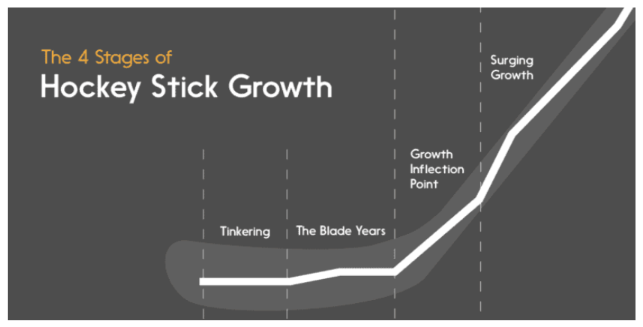
\includegraphics[scale=0.80]{images/hockey_stick.png}
\end{center}
Gli stadi principali di questa crescita sono:
\begin{itemize}
    \item \textbf{Tinkering stage};
    \item \textbf{The blade years};
    \item \textbf{Growth inflection point};
    \item \textbf{Surging growth}.   
\end{itemize}
Andiamo ora a studiarli singolarmente.

\newpage
\subsubsection{Tinkering stage, fase di avvio}

In questa fase gli imprenditori devono capire se la loro idea sia fattibile,
cercando anche di trovare il giusto equilibrio tra problemi e soluzioni. Il
tinkering termina quando si passa dalla teoria alla pratica.

Anche se questa fase non comporta molta pressione agli imprenditori, ci sono due
errori principali che potrebbero comunque mandare all'aria un'idea innovativa,
quali:

\begin{enumerate}
    \item Perdere troppo tempo nella costruzione di un business model accurato;
    \item Non cercare feedback sul prodotto/servizio per paura che l'idea venga
    copiata. 
\end{enumerate}
In questo momento l'attenzione deve essere rivolta alla sperimentazione e allo
sviluppo dell'offerta in base ai feedback ricevuti dai potenziali clienti.

\subsubsection{Blade years stage, fase di trazione}

I Blade years sono il periodo di tempo in cui viene convalidata l'idea sul
mercato, utilizzando versioni grezze, come l'MVP (Minumum Valuable Product) o la
versione beta, e in cui viene sviluppata l'idea finale e il relativo modello di
business. Solitamente in questa fase viene attuato il cosidetto
\textbf{bootstrapping}, ovvero cercare round d'investimenti per poter finanziare
il progetto. Ecco eventuali errori che un imprenditori potrebbe commettere
durante i blade years:

\begin{enumerate}
    \item Dedicare troppo tempo a raccogliere capitali per pagare le spese
    personali;
    \item Spendere troppo per le attività di vendita e marketing;
    \item Non essere disposti a modificare ulteriormente il prodotto.  
\end{enumerate}

\subsubsection{Growth inflection point, fase di scalabilità}

Qui ci troviamo al punto di svolta, il business model viene perfezionato e le
entrate dovrebbero cominciare a crescere in modo esponenziale. Gli imprenditori
possono sfruttare il loro slancio di crescita per attirare \textbf{venture
capitalist} o altri investitori.

Questa fase però presenta rischi significativi:

\begin{enumerate}
    \item Non riuscire a controllare la crescita dell'attività potrebbe \\
    portare ad un crollo;
    \item Pensando di sfruttare al massimo l'opportunità di crescita, si tende a
    modificare un prodotto che ha già funzionato fino a questo momento. 
\end{enumerate}
L'obiettivo principale deve essere quello di valutare attentamente le operazioni
e di sincronizzarle con la crescita dei ricavi.

\subsubsection{Surging growth stage, fase di maturità}

Una volta che la start-up si dimostra capace di sostenere la crescita
esponenziale durante lo stadio precedente, la sua crescita continua ad
accellerare a ritmo sostenuto, attirando sempre più clienti a provare l'offerta.

In questa fase, gli imprenditori devono affrontare le difficoltà che derivano
dall'esplosione di mercato, per questo si trovano davanti a tre scelte:

\begin{enumerate}
    \item Vendere l'azienda;
    \item Rimanere l'amministratore delegato;
    \item Assumere un amministratore delegato per gestire l'azienda. 
\end{enumerate}

\subsection{La start-up in Italia}

Nell'ordinamento giuridico in Italia è riconosciuta la \textbf{start-up
innovativa}. Queste start-up devono soddisfare almeno uno dei tre seguenti
punti:

\begin{enumerate}
    \item Almeno il 15\% del maggiore tra fatturato e costi annui deve essere
    rivolto ad attività di \textbf{ricerca e sviluppo};
    \item La forza lavoro è costituita per almeno un terzo da dottorandi, oppure
    da almeno due terzi da soci o collaboratori in possesso di laurea
    magistrale;
    \item L'impresa è titolare di un \textbf{brevetto o software registrato}.  
\end{enumerate}
Sono previsti incentivi per chi investe nelle start-up. Le persone fisiche hanno
il diritto a detrarre un importo pari al 30\% dell'investimento con un limite
massimo di 1 milione di euro annui, con un periodo minimo di mantenimento
dell'investimento pari a 3 anni.

Le società ottengono la stessa percentuale, con le stesse condizioni, ma con un
tetto massimo di 1 milione e 800 mila euro annui detraibili.

\subsection{La business idea}

Possiamo sintetizzare la messa a fuoco di un'idea di business con 3 passaggi
sequenziali:

\begin{enumerate}
    \item \textbf{Fase di analisi}, in cui si acquisiscono delle informazioni e
    \\ conoscenze sullo sviluppo del mercato nel quale ci si vuole inserire;
    \item \textbf{Fase creativa}, in cui si trasformano ed estrapolano le
    informazioni;
    \item \textbf{Fase della maturazione e della visione}, in cui si raffina
    l'idea. 
\end{enumerate}

\subsection{Il business model}

Il business model è l'insieme delle soluzioni organizzative e strategiche
attraverso le quali l'impresa acquisisce un vantaggio competitivo. Questo
modello deve avere 4 caratteristiche fondamentali, ovvero essere:

\begin{enumerate}
    \item \textbf{Sostenibile}: deve produrre reddito, ovvero generare ricavi
    maggiori dei costi;
    \item \textbf{Scalabile}: deve poter crescere velocemente, ricavi che
    crescono esponenzialmente a fronte di costi lineari;
    \item \textbf{Replicabile}: si deve poter replicare il modello su più paesi
    (ad esempio Uber, Netflix, Amazon);
    \item \textbf{Praticabile}: deve essere attuabile, non si può inventare
    qualcosa che non è attuabile (come la macchina del tempo).  
\end{enumerate}
uno degli errori più comuni è quello di presentare il business plan prima di
aver redatto il business model, in quanto quest'ultimo indica:
\begin{itemize}
    \item Che cosa;
    \item Quanto tempo;
    \item Quanti soldi;
\end{itemize}
servono per mettere in pratica il business model.

\newpage
\section{Lezione 6}

\subsection{I vari tipi di business model}

\subsubsection{Business model transazionale}

Questo tipo di business model rappresenta uno dei modelli \\più tradizionali e
diffusi nel panorama economico. Si basa sulla semplice ma efficace logica di
\textbf{vendere prodotti o servizi direttamente ai consumatori}, generando
ricavi attraverso le transazioni che avvengono durante gli acquisti.

\textcolor{red!50}{Come crea valore?}
L'azienda crea valore offrendo beni e servizi che soddisfano le esigenze
specifiche dei clienti. I ricavi derivano dalle vendite, che possono avvenire
tramite canali fisici, come negozi tradizionali, o piattaforme digitali. Questo
modello offre \textbf{flessibilità} nella definizione dell'offerta e la
possibilità di costruire \textbf{relazioni dirette con i clienti}. Però presenta
anche delle sfide, come \textbf{creare} un brand forte e lo \textbf{sviluppo} di
una strategia efficace di marketing.

\begin{center}
    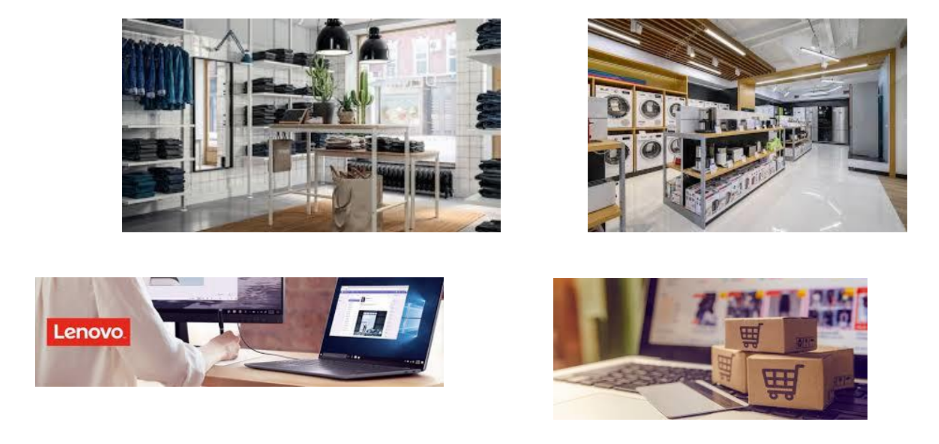
\includegraphics[scale=0.60]{images/transazionale.png}
    Esempio di modelli transazionali
\end{center}

\subsubsection{Business model marketplace}

Questo modello si basa sulla creazione di una \textbf{piattaforma} che funga da
intermediario tra venditore e cliente, facilitando le transazioni e creando
valore attraverso la conessione. In questo caso l'azienda non produce
direttamente i beni, offre solo l'infrastruttura e le regole che consentono agli
utenti di interagire efficacemente.

Il successo di un marketplace dipende dalla capacità di \textbf{attrarre e
mantenere} un numero sufficiente di utenti su entrambi i lati della piattaforma,
tramite elementi come la fiducia, la trasparenza e la qualità del servizio.

\begin{center}
    
\includegraphics[scale=0.50]{images/marketplace.png}
    Esempio di modelli marketplace
\end{center}

\newpage
\subsubsection{Business model SAAS (Software As A Service)}

Si basa sulla distribuzione di un software attraverso il cloud, con un sistema
di \textbf{abbonamento} che prevede pagamenti ricorrenti.

Il vantaggio principale di questo business è la facilità di acquisire e
fidelizzare clienti, in quanto un piccolo canone mensile/annuale non può essere
confrontato all'acquisto di software tradizionale.

Dal punto di vista del fornitore, questo modello garantisce \\un \textbf{flusso
di entrare più prevedibile e costante}, facilitando la pianificazione
finanziaria e gli investimenti in ricerca e sviluppo.

\begin{center}
    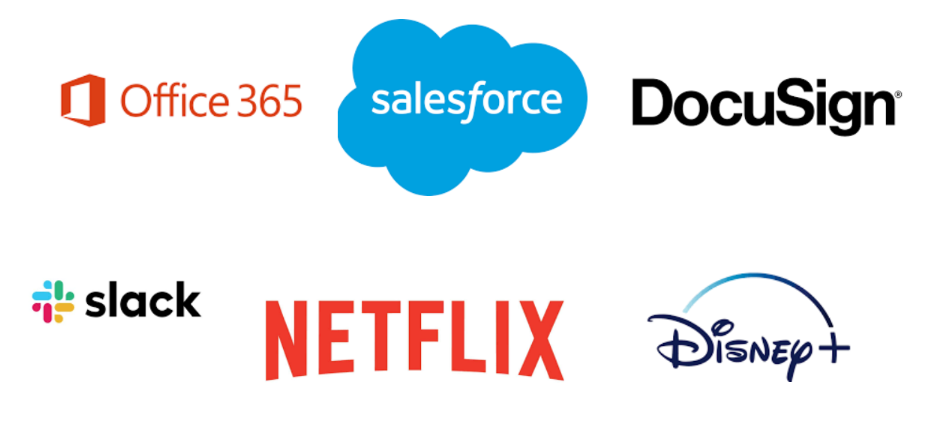
\includegraphics[scale=0.60]{images/saas.png}
    Esempio di modelli SAAS
\end{center}

\subsubsection{Business model freemium}

il modello freemium combina l'offerta gratuita di un prodotto o servizio di base
con opzioni \textbf{premium a pagamento}. Ci si basa sul principio di attrarre
un grande bacino di utenti tramite la prima versione senza costi, offrendo
successivamente \textbf{funzionalità aggiuntive o contenuti esclusivi} a coloro
che decidono di passare ad un piano a pagamento.

Tuttavia, l'implementazione di questo modello richiede un'attenta
pianificazione. Risulta fondamentale trovare il giusto equilibrio tra
funzionalità gratis e a pagamento:

\begin{itemize}
    \item L'offerta gratuita deve essere abbastanza allettante da attrarre
    clienti;
    \item Allo stesso tempo però deve essere abbastanza limitata da incentivare
    l'upgrade. 
\end{itemize}

\begin{center}
    
\includegraphics[scale=0.50]{images/freemium.png}
    Esempio di modelli freemium
\end{center}

\newpage
\subsubsection{Business model pay-as-you-go}

Questo modello si basa sul principio di far pagare al cliente il \\servizio o
prodotto solo in base all'effettivo utilizzo. Offre una grande
\textbf{flessibilità}, consentendo di personalizzare l'offerta in base alle
esigenze e possibilità specifiche di ciascun cliente

\begin{center}
    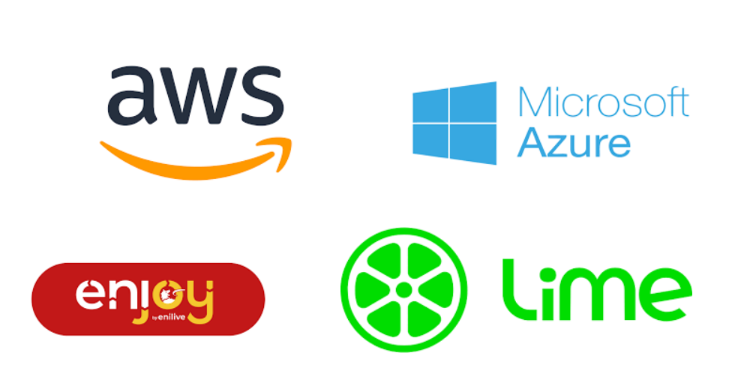
\includegraphics[scale=0.70]{images/payasyougo.png}
    Esempio di modelli pay-as-you-go
\end{center}

\subsubsection{Business model noleggio o leasing}

Questo modello si fonda sul \textbf{noleggio di beni o immobili}, tipicamente
per uso aziendale, in cambio del pagamento di un \textbf{canone periodico}.
Questo risulta particolarmente adatto ad aziende che offrono prodotti o servizi
ad alto costo, rendendoli accessibili ad un pubblico più ampio attraverso il
noleggio invece che l'acquisto diretto.

Il \textbf{vantaggio principale} è la capacità di generare flussi di cassa
stabili e prevedibili, oltre alla possibilità di instaurare un rapporto duraturo
con i clienti.

\begin{center}
    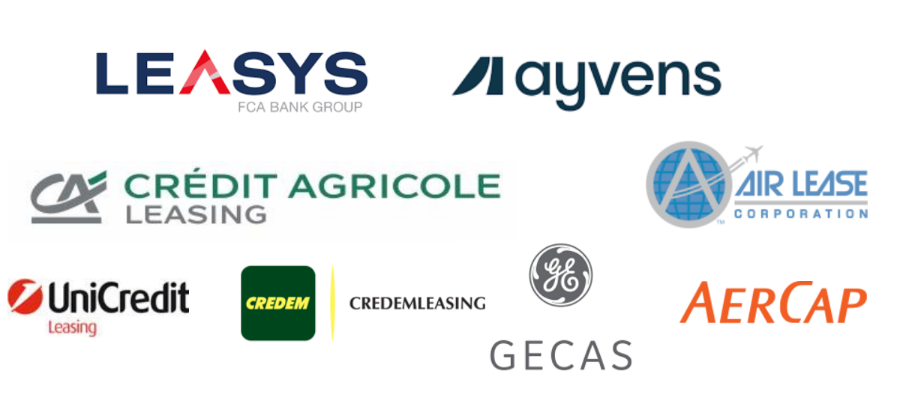
\includegraphics[scale=0.60]{images/noleggio.png}
    Esempio di modelli di noleggio o leasing
\end{center}

\subsubsection{Business model franchising}

Questo modello consente ad un'azienda di \textbf{espandere rapidamente la
propria presenza sul mercato} concedendo a terze parti, detti afffiliati o
\textbf{franchisee}, il diritto di utilizzare il proprio marchio e sistemi
operativi, situazione di win-win con chi vuole affiliarsi, in quanto troverà un
format di business già collaudato e riconosciuto.

\begin{center}
    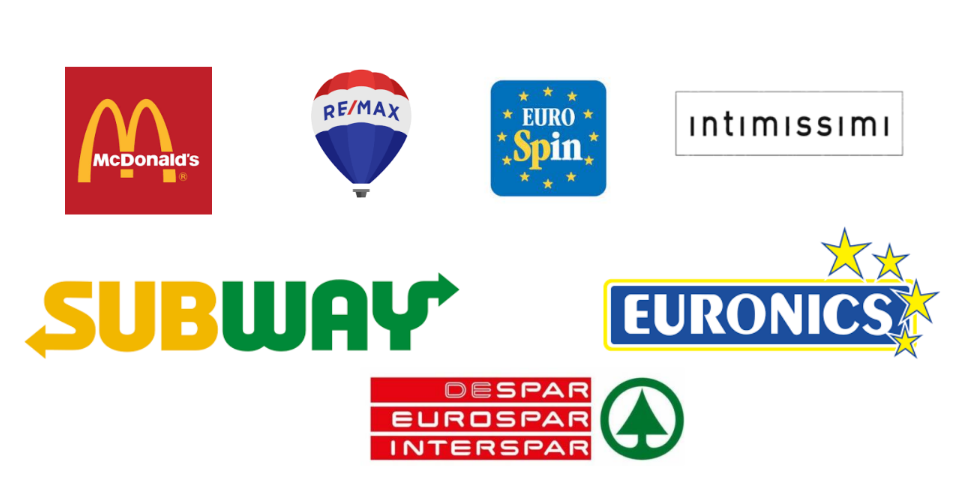
\includegraphics[scale=0.55]{images/franchising.png}
    Esempio di modelli franchising
\end{center}

\subsubsection{Business model broker}

I broker sfruttano la distanza fisica tra i venditori e i loro clienti. Si basa
sul fornire una piattaforma in cui acquirenti e venditori possano entrare in
contatto, facilitando le loro interazioni. La società gestisce le loro
transazioni e garantisce la sicurezza.

Le entrare in questo modello di business sono generate tramite l'applicazione di
piccole commissioni alle transazioni.

\begin{center}
    
\includegraphics[scale=0.55]{images/broker.png}
    Esempio di modelli broker
\end{center}

\subsubsection{Business model community}

La community rappresenta un approccio innovativo che sfrutta il \\potere delle
\textbf{connessioni sociali} e del \textbf{senso di appartenenza} per creare
valore. In questo modello l'azienda costruisce e gestisce una piattaforma o un
ambiente che facilita le interazioni con i membri, generando ricavi attraverso
vari meccanismi legati alla partecipazione alla community stessa.

il \textbf{valore aggiunto} di questo modello risiede nella capacità di creare
un \textbf{ecosistema autoalimentato}. Più la community cresce e si arricchisce
di contenuti e interazioni, più diventa attraente per nuovi membri.

\begin{center}
    
\includegraphics[scale=0.70]{images/community.png}
    Esempio di modelli community
\end{center}

\subsubsection{Business model affiliazione}

Un popolare modello di business sul web è quello delle affiliazioni. Funziona
promuovendo collegamenti a prodotti pertinenti, riscutendo commissioni sulle
vendite.

Uno dei vantaggi più evidenti di questo modello è che generalemente genera più
ricavi rispesso a modelli basati sulla pubblicità.

\begin{center}
    
\includegraphics[scale=0.80]{images/affiliazioni.png}
   
    Esempio di modelli di affiliazione
\end{center}

\newpage
\subsubsection{Business model inserzione}

In questo modello si ottengono dei ricavi senza richiedere un pagamento diretto
da parte degli utenti. Si fonda sull'idea di offrire gratuitamente un bene o una
piattaforma al pubblico, generando ricavi attraverso la \textbf{vendita di spazi
pubblicitari} a inserzionisti interessati a raggiungere quella specifica
audience.

il \textbf{vantaggio principale} di questo modello è che risulta più facile
avvicinare un ampio bacino di utenti, tuttavia serve \textbf{bilanciare
\\adeguatamente l'esperienza utente} con la necessità di monetizzazione. Un
eccesso di pubblicità può infatti allontanare gli utenti, compromettendo
l'efficacia del modello stesso.

\begin{center}
    
\includegraphics[scale=0.60]{images/inserzioni.png}
    Esempio di modelli inserzionistici
\end{center}

\subsubsection{Business model donazione}

Questo modello genera entrate tramite donazioni volontarie da \\parte dei
clienti che vogliono supportare il valore dall'organizzazione o servizio.

Questo fa sì che sia particolarmente adatto ad organizzazioni non profit,
piattaforme digitali o progetti con una forte componente sociale o culturale.

Tuttavia è importante notare che questo modello è spesso affiancato ad altre
fonti di reddito per garantire una maggiore stabilità finanziaria.

\begin{center}
    
\includegraphics[scale=0.60]{images/donazioni.png}
    Esempio di modelli a donazione
\end{center}

\section{Lezione 7}

\subsection{Il business model canvas}

Il business model viene descritto grazie a \textbf{9 blocchi base} che mostrano
la logica di come un'azienda intende produrre \textbf{valore}.

Questi 9 blocchi coprono le 4 aree principali di ogni business:

\begin{enumerate}
    \item Clienti;
    \item Offerta;
    \item Infrastruttura;
    \item Sostenibilità finanziaria.
\end{enumerate}

\subsubsection{Blocco 1, proposta di valore}

Questo blocco indica il pacchetto di prodotti e servizi che rappresenta un
\textbf{valore} per uno specifico \textbf{segmento di clientela}.

La proposta di valore non è altro che la \textit{reason why}, la ragione per la
quale i clienti scelgono un'azienda piuttosto che un'altra.

Questa sezione contraddistingue in maniera univoca il modello di business
aziendale determinando il suo \textbf{successo o insuccesso}.

vediamo qualche elemento che può contribuire alla creazione di valore per il
cliente:

\begin{itemize}
    \item La novità del prodotto;
    \item La performance;
    \item La personalizzazione;
    \item Il design;
    \item Lo status dell'azienda;
    \item Il prezzo conveniente;
    \item Riduzione dei costi/rischi;
    \item Accessibilità;
    \item Convenienza.
\end{itemize}

\subsubsection{Blocco 2, segmenti di clientela}

Il blocco dei segmenti di clientela descrive i \textbf{differenti gruppi di
persone o organizzazioni} ai quali l'azienda si rivolge.

Un'azienda deve prendere una decisione consapevole di quali segmenti servire e
quali ignorare, presa quest'ultima il business model dovrà essere accuratamente
costruito attorno ai \textbf{bisogni specifici} dei clienti target.

Vediamo ora qualche tipologia di segmenti di clientela:

\begin{itemize}
    \item \textbf{Mass market}, quando il business model non distingue diversi
    segmenti (Esempio: elettronica di massa con smartphone, tablet, pc, ecc.);
    \item \textbf{Niche market}, ci si rivolge ad una clientela specifica e
    specializzata (Esempio: il mercato del collezionismo);
    \item \textbf{Segmented market}, distinguere i clienti in base al loro
    potere di spesa o in base alle loro finalità;
    \item \textbf{Diversified market}, quando un'azienda serve due segmenti non
    correlati ognuno con i propri bisogni e problemi (Amazon);
    \item \textbf{Multi-sided platforms}, quando il business model si rivolge a
    due o più segmenti interdipendenti (Esempio: una carta di credito ha bisogno
    di tanti utilizzatori ma anche di tanti esercizi che la accettino).    
\end{itemize}

\subsubsection{Blocco 3, canali}

Questo blocco descrive come un'azienda \textbf{comunica} e \textbf{raggiunge} i
suoi segmenti di clientela per fornire una proposta di valore.

\textbf{Comunicazione, Distribuzione e canali di vendita} costituiscono
l'interfaccia dell'azienda con i suoi clienti.

Questi canali sono i \textbf{punti di contatto} che giocano un ruolo
fondamentale nell'esperienza del cliente, essi sono fondamentali per diverse
funzioni:

\begin{itemize}
    \item Sensibilizzare i clienti sui prodotti e servizi dell'azienda;
    \item Aiutare i clienti a valutare la proposta di valore;
    \item Permettere ai clienti di acquistare specifici prodotti o servizi;
    \item Offrire una proposta di valore;
    \item Fornire assistenza ai clienti dopo la vendita.   
\end{itemize}

\subsubsection{Blocco 4, relazioni con i clienti}

Descrive il \textbf{tipo di relazioni} che un'azienda stabilisce con gli
specifici segmenti di clientela. Un'azienda deve decidere che tipo di relazioni
stabilire con i propri clienti, relazioni che possono andare da quelle
\textbf{automatizzate} a quelle \textbf{personali}.

ci sono diverse categorie di relazioni con i clienti che possono co-esistere
nella relazione di un'azienda con un segmento di clientela:

\begin{itemize}
    \item Assistenza personale;
    \item Assistenza personale dedicata;
    \item Self-service;
    \item Automated services;
    \item Communities;
    \item Co-creazione.
\end{itemize}

\subsubsection{Blocco 5, flussi dei ricavi}

Qui vengono rappresentati i ricavi che l'azienda può generare da ogni segmento
di clientela.

Un business può includere due diversi tipi di flussi di ricavi:
\\\textbf{transazioni} o \textbf{pagamenti ricorrenti}.

quali sono più dettagliatamente questi flussi dei ricavi?

\begin{itemize}
    \item Vendita di un bene (asset sale);
    \item Tariffa d'uso (usage fee);
    \item Sottoscrizione (subscription fee);
    \item Affitto/leasing;
    \item Vendita di una licenza;
    \item Commissioni di intermediazione;
    \item Advertising;
\end{itemize}

\subsubsection{Blocco 6, risorse chiave}

Racchiude le risorse più importanti necessarie per far funzionare un modello di
business. Qualsiasi business necessita infatti di risorse, che permettono
all'azienda di creare e offrire l'offerta di valore, raggiungere i mercati,
mantenere le relazioni con i segmenti di clientela e generare dei ricavi.

Le risorse chiave possono rientrare nelle categorie seguenti:

\begin{itemize}
    \item \textbf{Risorse fisiche}: beni fisici come impianti, edifici, veicoli,
    ecc.;
    \item \textbf{Risorse intellettuali}: come brand, brevetti e marchi,
    partnership e database dei clienti;
    \item \textbf{Risorse umane}: fondamentali nei settori con alto bisogno di
    conoscenza o creatività;
    \item \textbf{Risorse finanziarieà}: liquidità, linee di credito o stock
    option.   
\end{itemize}

\subsubsection{Blocco 7, attività chiave}

Descrive le attività più importanti che un'azienda deve fare per far funzionare
il proprio modello di business.

categorie di attività chiave:

\begin{itemize}
    \item \textbf{produzione};
    \item \textbf{problem solving};
    \item \textbf{piattaforme/reti}.
\end{itemize}

\subsubsection{Blocco 8, partner chiave}

In questo blocco si trova il \textbf{network di fornitori e partner} che
un'azienda deve sviluppare per far funzionare il proprio modello di business.

Ci sono 4 tipi di partnership possibili:

\begin{enumerate}
    \item Alleanze strategiche tra aziende non competitors;
    \item Cooperazioni strategiche tra aziende competitors;
    \item Joiny ventures, per sviluppare nuovi business;
    \item Relazione acquirente-fornitore per assicurarsi forniture affidabili.   
\end{enumerate}

Queste partnership vengono create per diverse ragioni:

\begin{itemize}
    \item Ottimizzazione ed economie di scala;
    \item Riduzione dei rischi e dell'incertezza;
    \item Acquisizione di particolari risorse e attività.
\end{itemize}

\subsubsection{Blocco 9, struttura dei costi}

Descrive \textbf{tutti i costi da sostenere} per il funzionamento del business.

Questi costi sono facilmente individuabili una volta che sono state definite le
risorse chiave, le attività chiave e le partnership chiave. Ovviamente i costi
in qualsiasi business vanno minimizzati.

Si distinguono 2 classi di strutture dei costi:

\begin{enumerate}
    \item Cost-driven, ovvero business concentrati sulla minimizzazione dei
    costi ovunque possibile;
    \item Value-driven, business che si concentrano prima sulla creazione di
    valore. 
\end{enumerate}

\begin{center}
    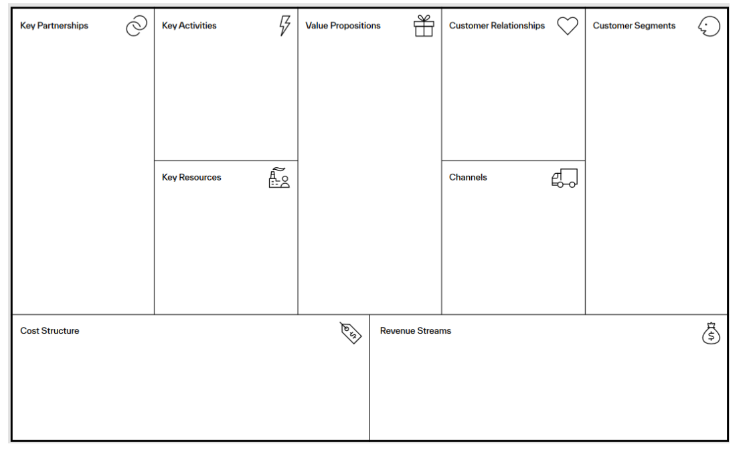
\includegraphics[scale=0.77]{images/businessmodelcanvas.png}
    Il business model canvas
\end{center}

\section{Lezione 8}

\subsection{Testare le idee di business}

L'errore più comune di imprenditori e innovatori è quello di partire con
\textbf{l'esecuzione senza evidenze}. Infatti risulta necessaria la validazione
dell'idea prima di partire con l'esecuzione, si deve dunque testare ampiamente
per evitare di sprecare tempo, energia e risorse in idee che non funzionano.

Per testare una business idea si \textbf{scompone in piccole ipotesi testabili}.
Queste ipotesi devono coprire tre tipi di rischi:

\begin{enumerate}
    \item \textbf{Desiderabilità}: I clienti potrebbero non essere interessati
    (Esempio: il mercato è troppo piccolo);
    \item \textbf{Fattibilità}; Non è possibile realizzare l'idea;
    \item \textbf{Sostenibilità}: L'idea non è sostenibile poiché non genera
    abbastanza ricavi.  
\end{enumerate}

Si segue un processo sequenziale e iterativo che prevede di:

\begin{itemize}
    \item Identificare le ipotesi chiave;
    \item Testare le ipotesi con gli esperimenti;
    \item Analizzare le evidenze e adattare l'idea ai risultati.
\end{itemize}

\begin{center}
    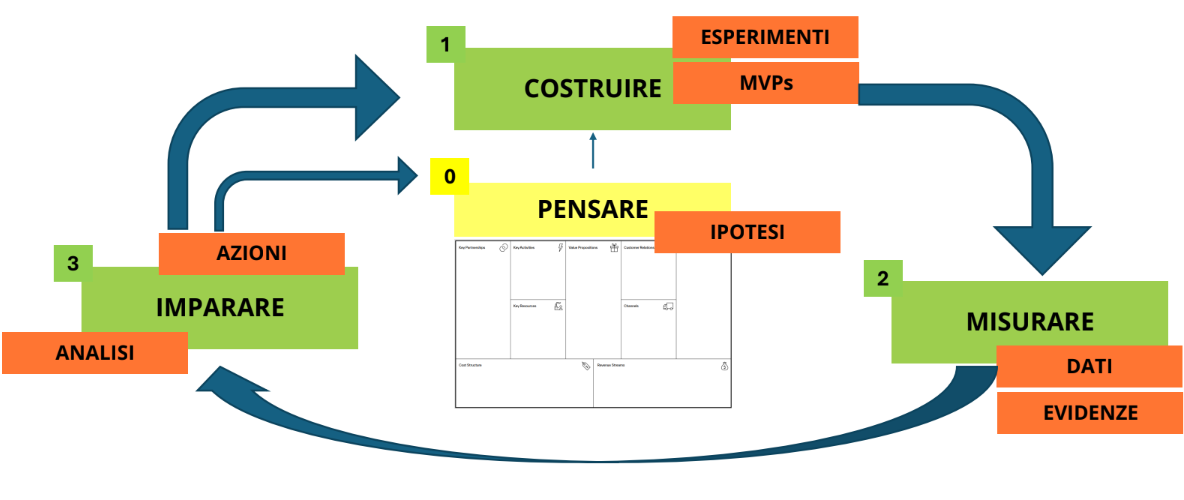
\includegraphics[scale=0.45]{images/testare.png}
    Mappa dei processi per testare un idea
\end{center}

\subsection{Ipotesi chiave}

Le ipotesi chiavi si concentrano sugli \textbf{aspetti del business}:

\begin{itemize}
    \item sono le ASSUNZIONI sulle quali è costruita la value proposition, il
    business model e le strategie;
    \item Sono gli ASPETTI DA ANALIZZARE per capire se la business idea può
    funzionare.
\end{itemize}

\newpage
Un'ipotesi di business ben formata descrive una cosa \textbf{testabile, precisa
e discreta} che si vuole investigare.

Le ipotesi chiave riguardano i rischi principali: \textbf{Desiderabilità,
Fattibilità e Sostenibilità}

\begin{center}
    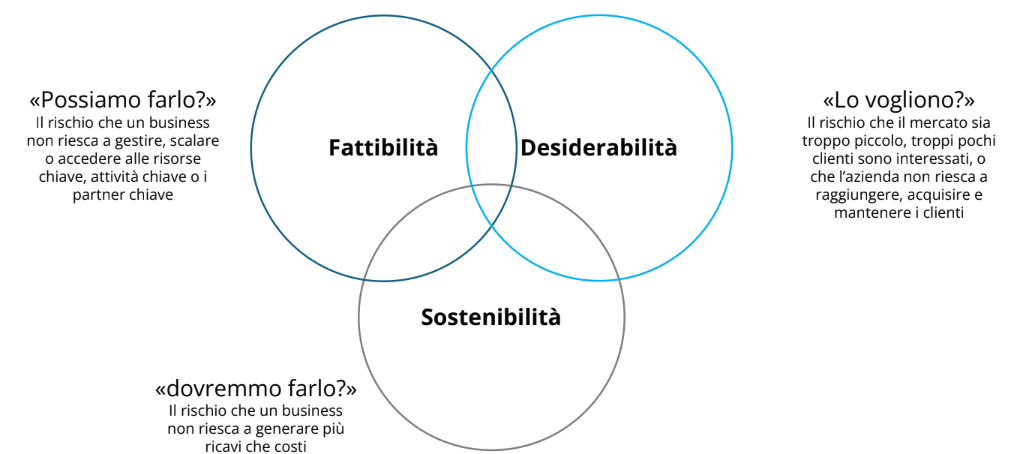
\includegraphics[scale=0.55]{images/rischi.png}
    Rischi principali

    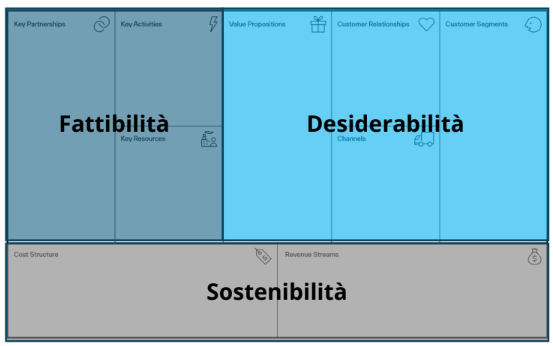
\includegraphics[scale=0.80]{images/ipotesi.png}
    
    Ipotesi chiave nel business model canvas
\end{center}

\section{Lezione 9}

\subsection{Progettazione della value proposition}

La value proposition è uno degli elementi fondamentali del business model canvas
e del business plan, richiede quindi un'attenzione particolare per la sua
definizione, con un approfondimento sui metodi che permettono di ottenere il
miglior risultato.

Come si definisce la value proposition? \\Per questo ci viene in aiuto un
modello messo a punto dagli stessi autori del business model canvas: il
\textbf{value proposition canvas}.

\subsection{Il value proposition canvas}

Il value proposition canvas ha due componenti:

\begin{enumerate}
    \item il profilo del cliente (\textbf{customer profile});
    \item la mappa del valore (\textbf{value map}). 
\end{enumerate}
con il profilo del cliente viene chiarita la percezione del cliente, mentre con
la mappa del valore si descrive come si intende creare valore.

L'obiettivo è raggiungere l'incastro tra i due componenti, quando gli elementi
di uno corrispondono agli elementi dell'altro, si cerca dunque di \textbf{creare
valore osservando i clienti}.

\begin{center}
    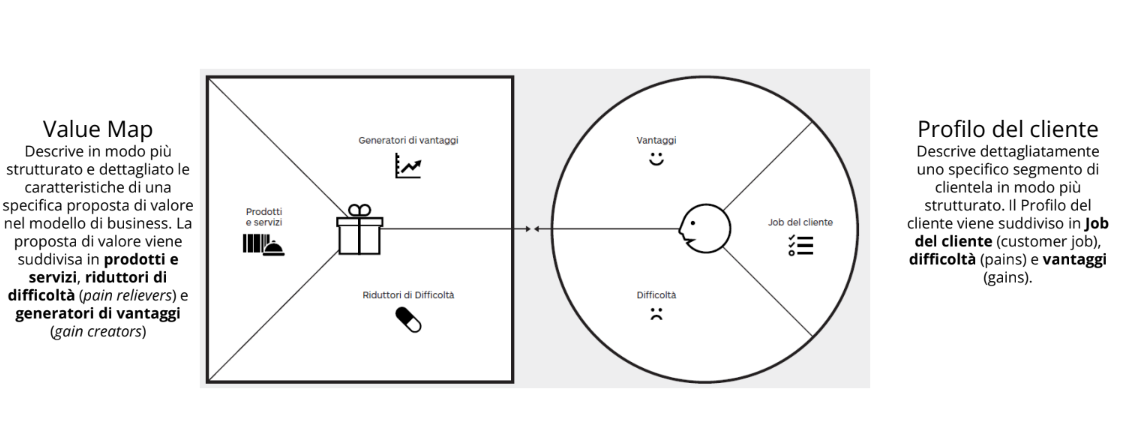
\includegraphics[scale=0.50]{images/valuecanvas.png}
    La value proposition canvas
\end{center}
Andiamo a sviscerare le componenti che possiamo vedere nella figura:

\begin{itemize}
    \item \textbf{Generatori di vantaggi}: descrive come i prodotti e servizi
    creano vantaggio per il cliente;
    \item \textbf{Prodotti e servizi}: Lista di tutti i prodotti e servizi su
    cui è costruita la value proposition;
    \item \textbf{Riduttori di difficoltà}: descrive come i prodotti e servizi
    \\
    riducono le difficoltà del cliente;
    \item \textbf{Vanttaggi}: descrive i risultati che il cliente vuole ottenere
    o quelli che sta cercando;
    \item \textbf{Job del cliente}: descrive cosa i clienti stanno cercando di
    ottenere nel loro lavoro o nella loro vita;
    \item \textbf{Difficoltà}: descrive i risultati negativi, i rischi e gli
    ostacoli connessi al job del cliente.
\end{itemize}

\newpage
\subsubsection{Profilo del cliente}

L'idea è quella di calarsi nei panni del cliente.

\textbf{OBIETTIVO}: visualizzare gli aspetti più importanti per i clienti in un
formato condivisibile.

\textbf{RISULTATO}: profilo del cliente in una pagina con elementi azionabili.

\subsubsection{La proposta di valore}

L'idea è sempre quella di calarsi nei panni dei clienti.

\textbf{OBIETTIVO}: descrivere esplicitamente come i prodotti e servizi creano
valore.

\textbf{RISULTATO}: proposta di valore in una pagina.

\newpage
\subsection{Adeguatezza value proposition-profilo cliente}

Una volta completati il profilo cliente e la value proposition si controlla
l'adeguatezza reciproca. Si raggiunge l'adeguatezza quando i clienti sono
entusiasti della vostra proposta di valore, il che accade quando affrontate un
job importante, alleviate diffoltà estreme e create vantaggi essenziali a cui i
clienti tengono.

\textbf{OBIETTIVO}: verificare se si sta affrontando ciò che interessa ai
clienti.

\textbf{RISULTATO}: connessione tra prodotti e servizi e i job, le difficoltà e
i vantaggi dei clienti.

\begin{center}
    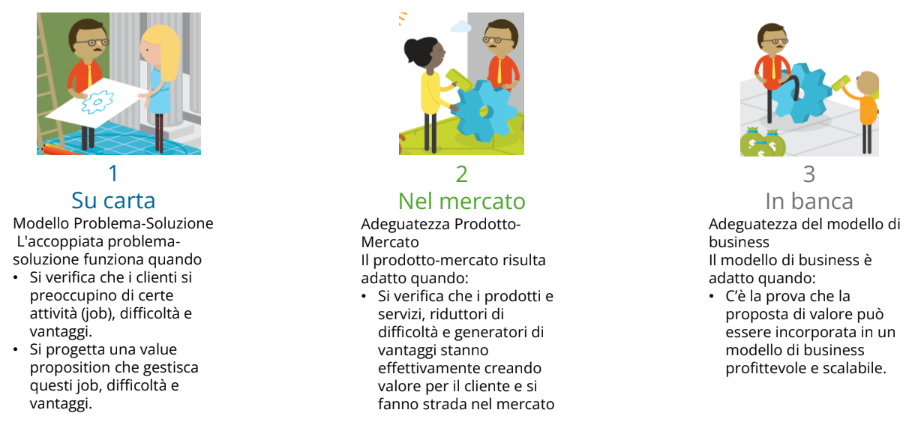
\includegraphics[scale=0.60]{images/adeguatezza.png}
    Tipi di adeguatezza
\end{center}

\section{Lezione 12}

\subsection{Il business plan}

Il business plan è uno strumento essenziale per chiunque voglia avviare o
sviluppare un'attività.

Con il business plan è possibile: 

\begin{itemize}
    \item Definire obiettivi chiari;
    \item Pianificare le strategie;
    \item Valutare la fattibilità economica.
\end{itemize}
Possiamo immaginare il business plan come una mappa che guida nel percorso
imprenditoriale, segnala le tappe fondamentali e aiuta a prevedere gli ostacoli
lungo il cammino.

\subsubsection{Executive summary}

Questa parte del business plan è fondamentale in quanto è la prima ad essere
esaminata dagli investitori, risulta essere un \textbf{biglietto da visita}.
L'obiettivo è catturare l'attenzione del lettore e comunicare in modo chiaro ed
efficace i punti chiave del progetto imprenditoriale. Spesso questa sezione
viene completata per ultima, quando ogni capitolo è stato attentamente
completato ed analizzato in tutto le sue parti.

\subsubsection{Il mercato di riferimento}

Sezione che esplicita a quale mercato si rivolge l'azienda e il prodotto o
servizio. Risulta fondamentale mostrare:

\begin{itemize}
    \item Dati attendibili da fonti terze (da citare);
    \item Numeri importanti o dei clienti potenziali o del giro d'affari
    potenziale;
    \item Trend. 
\end{itemize}
In genere vengono identificati:

\begin{itemize}
    \item \textbf{TAM} (Total Addresable Market), ovvero la domanda totale di un
    determinato prodotto o servizio;
    \item \textbf{SAM} (Served Addressable Market), ovvero il mercato
    potenzialmente disponibile;
    \item \textbf{SOM} (Servicealble \& Obtainable Market), ovvero il mercato
    che realisticamente potrebbe raggiungere l'azienda. 
\end{itemize}

\begin{center}
    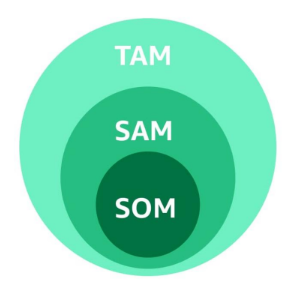
\includegraphics{images/mercato.png}
\end{center}

\subsubsection{Il problema}

In questa sezione vengono descritte le difficoltà dei clienti, come vengono
affrontate attualmente e perché le soluzioni attuali sono inefficienti. Il
problema deve essere descritto chiaramente, devono essere espressi anche i
termini economici relativi al problema. La base di partenza è rappresentata
dalla sezione \textbf{difficoltà} del profilo del cliente nel Value Proposition
Canvas.

\subsubsection{La soluzione}

Serve ora spiegare chiaramente cosa si propone come soluzione ai problemi
individuati. La spiegazione deve essere sintetica ma chiara evitando termini
tecnici o poco comprensibili. Vanno descritti benefici concreti che si portano
con la soluzione.

\subsubsection{USP, Unique Selling Proposition}

Questa è una delle sezioni più importanti, è necessario spiegare in maniera
chiara perché la proposta è unica, convincente e perché durerà nel tempo. Vanno
evidenziati chiaramente gli aspetti che comunicano che cosa vi rende così
speciali, cosa vi faccia funzionare, quali sono le vostre intuizioni. La base di
partenza è rappresentata dalle sezioni \textbf{vantaggi e riduttori di
difficoltà} nel Value Proposition Canvas insieme alla \textbf{value proposition}
del Business Model Canvas.

\newpage
\subsubsection{Competitor e Vantaggi competitivi}

Vanno individuati ed indicati:
\begin{enumerate}
    \item I principali competitor diretti ed indiretti;
    \item Quali sono i vantaggi competitivi rispetto ad essi.
\end{enumerate}
Il confronto con clienti, fornitori e referenti di associazioni permette di
ottenere preziosi ragguagli sulla concorrenza.

Importante in questa sezione anche la SWOT analysis:

\begin{center}
    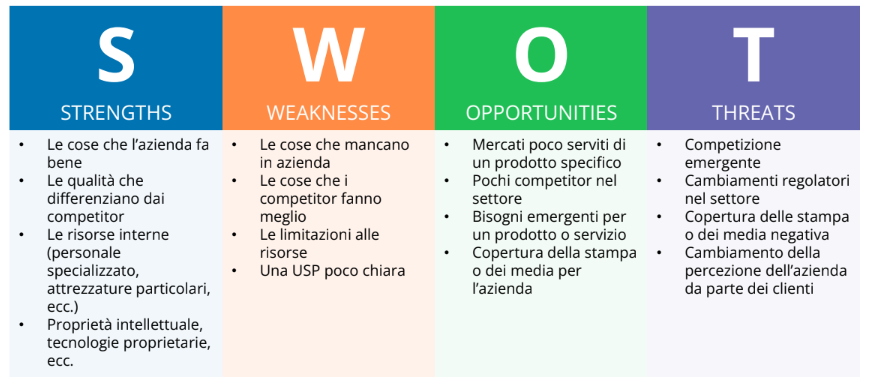
\includegraphics[scale=0.65]{images/SWOT.png}
\end{center}

\subsubsection{Business model, strategia di marketing e vendite}

Qui si esplicita quale business model si utilizza e a chi ci si rivolge, quale
strategia di marketing (eventi, adv online, influencer, ecc.) e quale strategia
di vendite (diretta, indiretta, mista, con distributori, ecc.)

\subsubsection{La roadmap}

In questa sezione si illustra come si pensa di sviluppare il prodotto di
vendita. Si utilizza una timeline con milestone più importanti per:

\begin{itemize}
    \item Prodotto;
    \item Clienti;
    \item Risultati tecnici fondamentali per lo sviluppo (certificazioni,
    prototipi, prima serie, ecc.).
\end{itemize}

\subsubsection{Il team}

Vengono presentati i principali componenti del team con le esperienza rilevanti
ai fini del progetto. Buona idea inserire le foto dei componenti, che permettono
al lettore di dare dei volti al progetto. Per ogni componente si indica il
ruolo, le capacità ed esperienze che lo rendono la persona giusta all'interno
del team.

\subsubsection{Il piano economico finanziario}

In questa sezione verranno mostrate le proiezioni economico finanziarie a 5 anni
con ricavi, costi ed ebitda. Buona pratica è utilizzare grafici per le
proiezioni.ù

\subsubsection{La richiesta e l'utilizzo dei fondi}

In questa parte si può trovare l'importo totale dei fondi necessari al piano di
sviluppo e quale è l'importo richiesto dalla società all'investitore finanziario
e quale è il timing di utilizzo dei capitali richiesti. Si deve comunicare in
modo chiaro e diretto:

\begin{itemize}
    \item L'importo dei fondi richiesto;
    \item Il loro utilizzo nel corso del tempo;
    \item I risultati che si raggiungono con i fondi.
\end{itemize}
Tutto per far capire come viene creato valore con i fondi impiegati.


\end{document}